\documentclass[tikz,crop]{standalone}

% Part of the preamble, for TikZ figures.
% This is used in both the main document and in the subfigures.
% One exception is minted: since the path depends on the file, it is not set.
\usepackage{tikz}
\usepackage{xcolor}
\usepackage{pgfplots}
\usepackage{tikz-uml}

\pgfplotsset{compat=1.18}
\usepgfplotslibrary{statistics}

\usetikzlibrary{shapes,arrows,positioning,backgrounds,calc,intersections,calc,svg.path}

\definecolor{ugent-re}{RGB}{220, 78, 40}        % vermilion			/ vermiljoen
\definecolor{ugent-we}{RGB}{45, 140, 168}       % no match
\definecolor{ugent-ge}{RGB}{232, 94, 113}       % rose				/ bleekrood
\definecolor{ugent-ea}{RGB}{111, 113, 185}      % distant blue		/ verblauw
\definecolor{ugent-pp}{RGB}{251, 126, 58}       % deep orange		/ dieporanje
\definecolor{ugent-ps}{RGB}{113, 168, 96}       % yellow green		/ geelgroen

\tikzstyle{python}=[fill=ugent-ps!50!white]
\tikzstyle{java}=[fill=ugent-we!50!white]
\tikzstyle{haskell}=[fill=ugent-ea!50!white]
\tikzstyle{js}=[fill=ugent-pp!50!white]
\tikzstyle{c}=[fill=ugent-re!50!white]

\newlength{\block}
\setlength{\block}{0.75cm}

\tikzstyle{a}=[anchor=north west]
\tikzstyle{box}=[a,draw,rectangle]
\tikzstyle{node}=[a,draw,minimum height=0.5cm,align=center,fill=white,text depth=.25ex]
\tikzstyle{document}=[node,tape,tape bend top=none]
\tikzstyle{cont}=[box,minimum height=1\block,minimum width=1\block]
\tikzstyle{arrow}=[draw, -latex]
\tikzstyle{inner}=[box,draw=gray]

% Blue box style
\tikzstyle{bluebox}=[draw=ugent-we,java]
\tikzstyle{redbox}=[draw=ugent-re,c]
\tikzstyle{greenbox}=[draw=ugent-ps,python]

% Some things specific to TESTed imagery.
\tikzstyle{tc}=[box,draw=ugent-ps]
\tikzstyle{comp}=[box,draw=ugent-re,fill=ugent-re,fill opacity=0.05]
\tikzstyle{exec}=[box,draw=ugent-we,fill=ugent-we,fill opacity=0.10]

% Stuff from tested-engine/concept.tex
\tikzstyle{process}=[node,rectangle]
\tikzstyle{terminator}=[node,rectangle,rounded corners=0.5cm]
\tikzstyle{io}=[node,trapezium,trapezium left angle=70,trapezium right angle=-70,minimum width=2.5cm,trapezium stretches=true]
\tikzstyle{small}=[font=\footnotesize,color=darkgray]
\tikzstyle{submission}=[document,align=right,minimum width=3cm,minimum height=1cm,text depth=0.5cm,inner sep=0.5mm,font=\scriptsize]

% Stuff from chatper3/flow.tex
\tikzstyle{height}=[minimum height=0.75\block]
\tikzstyle{contt}=[cont,minimum height=0.75\block]
\tikzstyle{compop}=[comp,text opacity=1]
\tikzstyle{execop}=[exec,text opacity=1]

\tikzstyle{hnode}=[draw,anchor=center,minimum height=\block,text depth=.25ex,align=center]
\tikzstyle{executable}=[hnode,ultra thick,fill=gray!10]
\tikzstyle{inner-exec}=[node,anchor=center,minimum width=3.25\block,densely dotted,font=\footnotesize,fill=none]
\tikzstyle{stmt}=[node,anchor=center,fill=gray!30,minimum width=4.5\block,font=\footnotesize]
\tikzstyle{fieldset}=[minimum height=\block,fill=white,text depth=.5ex,fill=white]

\definecolor{c9ed9e6}{RGB}{158,217,230}
% TODO: create better version of this, or use PDF directly...
\newcommand*\drawtesttube{%
    \kern0.2em\relax
    
\begin{tikzpicture}[scale=0.5,baseline=3pt,rotate=100]
%        \path[fill=c9ed9e6] (0.926, -0.5821)arc(229.9677:328.957:0.1058).. controls (1.1377, -0.5027) and (1.1113, -0.4498) .. (1.0583, -0.3969) -- (0.5821, -0.0265)arc(49.3987:229.3987:0.122) -- (0.4498, -0.2117) -- (0.0794, -0.7144)arc(143.1301:233.1301:0.2646) -- (0.1852, -1.1113)arc(232.7082:275.401:0.2646).. controls (0.4498, -1.1642) and (0.5027, -1.1113) .. (0.5556, -1.0583) -- (0.926, -0.5821) -- cycle(0.3704, -0.926) -- (0.3175, -0.926) -- (0.2646, -0.8996) -- (0.2646, -0.8467) -- (0.635, -0.3704) -- (0.7408, -0.4498) -- (0.3704, -0.926) -- cycle;
        \draw[fill=c9ed9e6,draw=none] svg {M35.043,22.196c0.813,0.616,1.77,0.915,2.717,0.915c1.358,0,2.703-0.615,3.589-1.783c1.501-1.98,1.111-4.803-0.868-6.305
			L21.868,0.915c-1.981-1.503-4.803-1.113-6.304,0.867s-1.113,4.804,0.868,6.305l0.254,0.192L2.776,26.633
			c-1.623,2.144-2.315,4.788-1.948,7.45c0.367,2.663,1.749,5.021,3.889,6.643l2.068,1.568c1.767,1.34,3.877,2.045,6.057,2.045
			c0.462,0,0.927-0.031,1.392-0.096c2.663-0.365,5.023-1.747,6.647-3.89L34.79,22.001L35.043,22.196z M13.709,34.918
			c-0.22,0.29-0.502,0.383-0.701,0.41c-0.201,0.026-0.496,0.014-0.785-0.205l-2.07-1.57c-0.289-0.218-0.381-0.5-0.409-0.697
			s-0.014-0.494,0.205-0.783l13.91-18.355l3.759,2.85L13.709,34.918z};
    \end{tikzpicture}%
    \kern0.2em\relax\space
}

% Minted environments for use in Tikz
\newminted[tikzjava]{java}{autogobble,linenos=false,fontsize=\tiny,stripall}
\newminted[tikzpython]{python}{autogobble,linenos=false,fontsize=\tiny,stripall}
\newminted[tikztext]{text}{autogobble,linenos=false,fontsize=\tiny,stripall}




\begin{document}

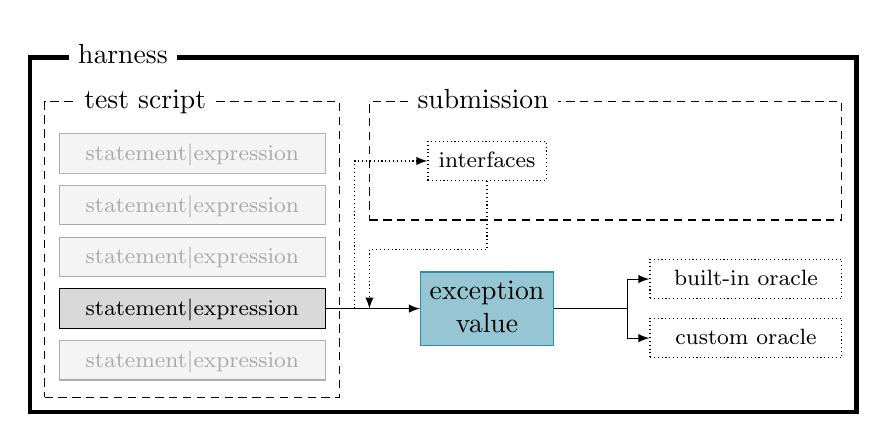
\begin{tikzpicture}[x=0.75cm,y=0.75cm,fill fraction/.style={path picture={
  \fill[#1]
  (path picture bounding box.west) rectangle
  (path picture bounding box.south east);
}},
  fill fraction/.default=gray!50]

  \node[hnode,ultra thick,label={[fieldset,above left=-0.54\block and 4.5\block]harness},minimum width=14\block,minimum height=6\block] at (6, 3) (harness) {};

  \node[inner-exec,densely dashed,anchor=center,fill=none,minimum width=5\block,minimum height=5\block,label={[fieldset,above left=-0.52\block and -0.4\block]test script}] at (1.75,2.75) (testsc) {};

  \node[stmt,opacity=0.3] at (testsc|-0,4.375) (testsc1) {statement\textbar{}expression};
  \node[stmt,opacity=0.3] at (testsc|-0,3.5) (testsc2) {statement\textbar{}expression};
  \node[stmt,opacity=0.3] at (testsc|-0,2.625) (testsc3) {statement\textbar{}expression};
  \node[stmt] at (testsc|-0,1.75) (testsc4) {statement\textbar{}expression};
  \node[stmt,opacity=0.3] at (testsc|-0,0.875) (testsc5) {statement\textbar{}expression};

  \node[inner-exec,densely dashed,minimum width=8\block,minimum height=2\block,label={[fieldset,above left=-0.52\block and 0.8\block]submission}] at (8.75,4.25) (subm) {};

  \node[inner-exec, anchor=center,left=1\block of subm.center,fill=none,minimum width=2\block] (interface) {interfaces};

  \node[hnode,minimum width=2\block,bluebox] at (interface|-testsc4) (out) {exception\\value};
  \draw[arrow] (testsc4) -- (out);

  \draw[arrow,densely dotted] (out-|4.5,0) |- (interface);

  \draw[arrow,densely dotted] (interface) |- (out|-0,2.75) -| (out-|4.75,0);

  \node[inner-exec] at (11.125,2.25) (mor) {built-in oracle};
  \node[inner-exec] at (11.125,1.25) (cor) {custom oracle};

  \draw[arrow] (out) -| (mor.west-|9.125,0) -- (mor);
  \draw[arrow] (out) -| (cor.west-|9.125,0) -- (cor);


%  \node[hnode,minimum width=2\block,greenbox] at (0, 0) (stdin) {stdin};
%
%  \node[executable,label={[label distance=-0.44cm,anchor=south,fill fraction=gray!30,fill=white,text depth=.5ex]127:submission},minimum width=4\block,minimum height=1.5\block] at (3.75, 0) (subm) {};
%  \draw[arrow] (stdin) -- (subm);
%  \node[inner-exec, anchor=center,below=0mm of subm.center, anchor=center, fill=none] (main) {main};
%
%  \node[hnode,minimum width=2\block,bluebox] at (7.5, 0) (out) {stdout\\stderr};
%  \draw[arrow] (subm) -- (out);
%
%  \node[executable,minimum width=4\block,minimum height=1.5\block] at (11.5, 1) (builtin) {};
%  \node[executable,minimum width=4\block,minimum height=1.5\block] at (11.5, -1) (custom) {};
%
%  \node[inner-exec, anchor=center,below=0mm of builtin.center, anchor=center, fill=none] (mor) {built-in oracle};
%  \node[inner-exec, anchor=center,below=0mm of custom.center, anchor=center, fill=none] (cor) {custom oracle};
%
%  \draw[arrow] (out) -| (builtin.west-|9,0) -- (builtin);
%  \draw[arrow] (out) -| (custom.west-|9,0) -- (custom);

\end{tikzpicture}

\end{document}
